%!TEX program = xelatex
\documentclass[aspectratio=169]{beamer}
\usefonttheme[onlymath]{serif}
\usepackage{blindtext}
\usepackage{bm}
\usepackage{minted}
\usepackage{amsmath, amssymb}
\usepackage{tikzsymbols}
\usepackage[linesnumbered,ruled,vlined]{algorithm2e}
\newcommand\blfootnote[1]{%
  \begingroup
  \renewcommand\thefootnote{}\footnote{#1}%
  \addtocounter{footnote}{-1}%
  \endgroup
}

\usetheme{Execushares}

\title{Risk Parity: Convex, Non-convex, and Hierarchical Models}
\subtitle{a talk by}
\author{\textbf{Vin\'icius}}
\date{May 15th, 2020}

\setcounter{showSlideNumbers}{1}

\begin{document}
	\setcounter{showProgressBar}{0}
	\setcounter{showSlideNumbers}{0}

	\frame{\titlepage}

        \begin{frame}
          \frametitle{Contents}
              \vspace{.5cm}
          \begin{enumerate}
            \item Markowitz and Portfolio Optimization
             \\ \textcolor{ExecusharesGrey}{\footnotesize\hspace{1em} Modern Portfolio Theory 101}
            \item Risk Parity Portfolio
             \\ \textcolor{ExecusharesGrey}{\footnotesize\hspace{1em} Historical events, convex, non-convex formulations,
             and bleeding-edge solvers in $\mathsf{R}$ and $\mathsf{Python}$}
            \item Hierarchical Risk Parity
              \\ \textcolor{ExecusharesGrey}{\footnotesize\hspace{1em} Combining graph theory and portfolio design}
            \item Conclusions
              \\ \textcolor{ExecusharesGrey}{\footnotesize\hspace{1em} Some closing thoughts}
          \end{enumerate}
        \end{frame}



	\setcounter{showSlideNumbers}{0}
        \section{Modern Portfolio Theory}
	\setcounter{framenumber}{0}
	\setcounter{showProgressBar}{1}
	\setcounter{showSlideNumbers}{1}

		\begin{frame}
			\frametitle{Modern Portfolio Theory}
                        \vspace{1cm}
                        \begin{itemize}
                          \item problem: how to allocate $B$ amount of money into $N$ assets?
                            \pause
                          \item assume the log-returns $\bm{r}$ are i.i.d. Gaussian, then for a portfolio $\bm{w}$:
                            \begin{itemize}
                              \item expected return: $\mathbb{E}\left[\bm{w}^\top \bm{r}\right] = \bm{w}^\top\boldsymbol{\mu}$
                              \item variance: $\mathbb{V}\left[\bm{w}^\top \bm{r}\right]$ = $\bm{w}^\top\boldsymbol{\Sigma}\bm{w}$
                            \end{itemize}
                            \pause
                          \item Dr. Harry Markowitz\footnote{1990 Nobel Memorial Prize in Economic Sciences} (1952):
                                  \begin{equation*}
                                  \begin{array}{ll}
                                    \underset{\bm{w}}{\textsf{maximize}} & \bm{w}^\top\boldsymbol{\mu} - \lambda\bm{w}^\top\boldsymbol{\Sigma}\bm{w}\\
                                    \textsf{subject to} & \bm{w}\succeq \mathbf{0}, ~\mathbf{1}^\top\bm{w} = 1
                                  \end{array}
                                  \end{equation*}
                            \pause
                           \item criticisms:
                             \begin{enumerate}
                               \item sensitivity to estimation errors in $\boldsymbol{\mu}$ and $\boldsymbol{\Sigma}$
                               \item does not consider risk diversification
                               \end{enumerate}
                        \end{itemize}
                        \blfootnote{  }
		\end{frame}

	\setcounter{showSlideNumbers}{0}
        \section{Risk Parity}
	\setcounter{framenumber}{1}
	\setcounter{showSlideNumbers}{1}

		\begin{frame}
			\frametitle{From Capital to Risk Allocation}
			\begin{itemize}
                          \item allocate \textbf{risk} rather than \textbf{capital} \vspace{.5cm}
                            \pause
                                \item first risk parity fund (1996): Bridgewater's All Weather \vspace{.5cm}
                            \pause
                                \item Bridgewater publishes "Engineering Targeted Returns and Risks" (2004) \vspace{.5cm}
                            \pause
                                \item 2011-onwards: risk parity gains broad adoption \vspace{.5cm}
                                  % adopted by many institutional investors
                            \pause
                                \item \textbf{basic idea}: design a portfolio such that the risk is equally distributed among the asset classes (stocks, bonds, real state,
                                  etc.)
			\end{itemize}
		\end{frame}

                \begin{frame}[fragile]
                  \frametitle{From Capital to Risk Allocation}
                  \vspace{1cm}
                  \begin{center}
                    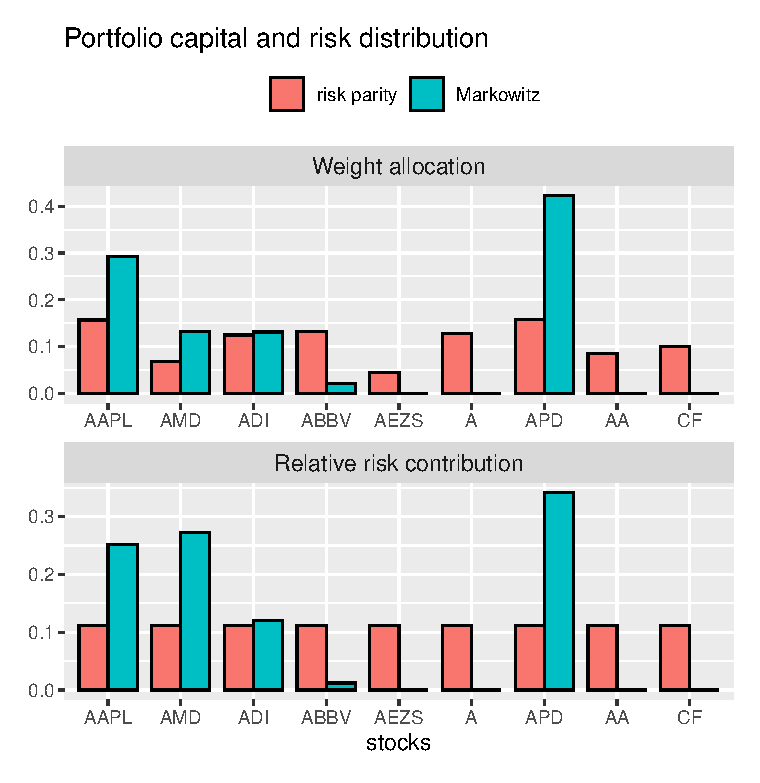
\includegraphics[scale=.62]{codes/markowitz-rpp-comparison.eps}
                  \end{center}
                \end{frame}

        \begin{frame}
            \frametitle{Problem Formulation}
            \vspace{.5cm}
            \begin{itemize}
              \item volatility:
                $\sigma(\bm{w}) = \sqrt{\bm{w}^\top\boldsymbol{\Sigma}\bm{w}}$
              \item from Euler's theorem:
                \begin{equation*}\sigma(\bm{w}) = \sum_{i} w_i \dfrac{\partial \sigma(\bm{w})}{\partial w_i}
                = \sum_{i} \dfrac{w_i \left(\boldsymbol{\Sigma}\bm{w}\right)_{i}}{\sqrt{\bm{w}^\top\boldsymbol{\Sigma}\bm{w}}} \end{equation*}
              \item $\dfrac{\partial \sigma(\bm{w})}{\partial w_i}$: \textbf{marginal risk contribution}
              \item measures the sensitivity of the portfolio volatility to the $i$-th asset
              \item it can be defined for other risk measures like VaR and CVaR
            \end{itemize}
        \end{frame}

        \begin{frame}
          \frametitle{Problem Formulation}
          \vspace{.75cm}
          \begin{itemize}
            \item \textbf{risk contribution} of the $i$-th asset to the total risk $\sigma(\bm{w})$:
              \begin{equation*}
                \textsf{RC}_{i} = w_i \dfrac{\partial \sigma(\bm{w})}{\partial w_i}
              \end{equation*}
            \item from Euler's theorem:
              \begin{equation*}
                \sum_{i}\textsf{RC}_i = \sigma(\bm{w})
              \end{equation*}
            \item \textbf{relative risk contribution} of the $i$-th asset to the total risk $\sigma(\bm{w})$:
              \begin{equation*}
                \textsf{RCC}_i = \dfrac{\textsf{RC}_i}{\sigma(\bm{w})} = \dfrac{w_i\left(\boldsymbol{\Sigma\bm{w}}\right)_i}{\bm{w}^\top\boldsymbol{\Sigma}\bm{w}},
              \end{equation*}
              so that
              \begin{equation*}
                \sum_{i}\textsf{RCC}_i = 1
              \end{equation*}
          \end{itemize}
        \end{frame}

        \begin{frame}
          \frametitle{Risk Parity: Problem Formulation}
          \vspace{.5cm}
            \begin{itemize}
              \item \textbf{risk parity portfolio}: $\textsf{RCC}_i = b_i,~i=1,2,\dots,N$
              \item \textbf{feasibility} problem:
            \begin{equation*}
            \begin{array}{ll}
              \underset{\bm{w} \succ \mathbf{0}}{\textsf{find}} & \bm{w} \\
              \textsf{subject to} &
              \dfrac{w_i\left(\boldsymbol{\Sigma\bm{w}}\right)_i}{\bm{w}^\top\boldsymbol{\Sigma}\bm{w}} =
              b_i,~ i = 1, 2, \dots, N
            \end{array}
            \end{equation*}
            doesn't look trivial
          \item \textbf{approximation}: $\boldsymbol{\Sigma}$ is diagonal
            \begin{equation*}
              w_i \propto \dfrac{\sqrt{b_i}}{\sqrt{\boldsymbol{\Sigma}_{ii}}}
            \end{equation*}
          i.e. \textbf{inverse volatility portfolio}
            \end{itemize}
        \end{frame}

        \begin{frame}
          \frametitle{Solution to Risk Parity}
          \vspace{.5cm}
          \begin{itemize}
            \item Spinu (2013):
            \begin{itemize}
            \item change of variables $\bm{x} = \dfrac{\bm{w}}{\sqrt{\bm{w}^\top\boldsymbol{\Sigma}\bm{w}}}$, then $\bm{w} = \dfrac{\bm{x}}{\mathbf{1}^\top\bm{x}}$
            \item problem becomes: $\boldsymbol{\Sigma}\bm{x} = \dfrac{\bm{b}}{\bm{x}}$
            \item $\underset{\bm{x} \succ \mathbf{0}}{\textsf{minimize}} ~f(\bm{x}) = \dfrac{1}{2}\bm{x}^\top\boldsymbol{\Sigma}\bm{x} - \bm{b}^\top\log(\bm{x})$
            \item \textbf{optimality condition:} $\nabla f(\bm{x}) = \boldsymbol{\Sigma}\bm{x} - \dfrac{\bm{b}}{\bm{x}} = \mathbf{0}$
            \item then done? it's not a QP, LP, etc.
           \end{itemize}
          \end{itemize}
        \end{frame}

        \begin{frame}{Cyclical Coordinate Descent (CCD)}
          \vspace{.5cm}
          Griveau-Billion (2013):

          \begin{algorithm}[H]
            \SetAlgoLined
            \caption{CCD to solve risk parity}
            $k \leftarrow 0$, initial $\bm{x}^{(0)}$\\
            \While{not converged}{
              \For{$i = 1$ to $N$}{
                $x_i^{k+1} \leftarrow \underset{x_i}{\textsf{arg min}} f\left(x_{1}^{k+1}, \dots, x_{i}^{k},
                \dots, x_{N}^{k}\right)$
              }
            }
          \end{algorithm}
          \begin{itemize}
            \item closed-form update:
          \end{itemize}
          \begin{equation*}
            x_i^\star = \frac{-\left(\bm{x}_{-i}^\top\boldsymbol{\Sigma}_{:,i}\right)+\sqrt{\left(\bm{x}_{-i}^\top\boldsymbol{\Sigma}_{:,i}\right)^2+
            4\boldsymbol{\Sigma}_{ii}b_i}}{2\boldsymbol{\Sigma}_{ii}},
          \end{equation*}
          where $\bm{x}_{-i} = \left[x_1, \dots, x_{i-1}, 0, x_{i+1}, \dots, x_{N}\right]^\top$
        \end{frame}

        \begin{frame}{Non-convex Formulations}
          \vspace{.5cm}
          \begin{itemize}
            \item limitations of the previous formulation: $\bm{w} \succ \mathbf{0}$, $\mathbf{1}^\top\bm{w} = 1$
            \pause
            \vspace{.25cm}
            \item in practice we would like to include $\bm{l} \preceq \bm{w} \preceq \bm{u}$, $\bm{w}^\top\boldsymbol{\mu}$
            \pause
            \vspace{.25cm}
            \item Bruder \& Roncalli (2012):
              \begin{equation*}
              \begin{array}{ll}
                \underset{\bm{w}}{\textsf{minimize}} &
                \sum_{i=1}^{N}\left(\dfrac{w_i(\boldsymbol{\Sigma}\bm{w})_i}{\bm{w}^\top\boldsymbol{\Sigma}\bm{w}} - b_i\right)^2\\
                \textsf{subject to} & \mathbf{1}^\top\bm{w} = 1, ~\bm{w} \in \mathcal{W}
              \end{array}
              \end{equation*}
            \vspace{.25cm}
            \pause
            \item how to "solve" the non-convex formulation?
            \vspace{.25cm}
            \pause
            \item general purpose solvers: slow \Sadey
            \end{itemize}
        \end{frame}

        \begin{frame}{Non-convex Formulations}
            \vspace{.5cm}
          \begin{itemize}
            \item Feng \& Palomar (2015):
              \begin{equation*}
              \begin{array}{ll}
                \underset{\bm{w}}{\textsf{minimize}} &
                \sum_{i=1}^{N}\left[g_{i}(\bm{w})\right]^2 + \lambda F(\bm{w})\\
                \textsf{subject to} & \mathbf{1}^\top\bm{w} = 1, ~\bm{w} \in \mathcal{W}
              \end{array}
              \end{equation*}
            \end{itemize}
            \begin{itemize}
            \pause
            \item "convexify" the objective function: fast \Laughey
            \vspace{.25cm}
            \pause
            \item \textbf{basic idea}: find a "nice" approximation to the non-convex term, solve it, repeat (Scutari et al. 2014)
            \vspace{.25cm}
            \pause
            \item "nice" approximation for $g_i(\bm{w})$: first order Taylor expansion (Feng \& Palomar 2015)
          \end{itemize}
        \end{frame}

        \begin{frame}{Open Source Software Packages}
          \begin{itemize}
            \item[] \includegraphics[scale=.1]{images/github.png}  dppalomar/riskParityPortfolio (R version)
            \item[] \includegraphics[scale=.1]{images/github.png} dppalomar/riskparity.py (Python version)
          \end{itemize}
          \begin{figure}[!htb]
            \centering
            \includegraphics[scale=0.1]{images/r.png}~
            \includegraphics[scale=0.2]{images/python.png}
          \end{figure}
        \end{frame}

        \begin{frame}[fragile]
          \frametitle{Basic Usage}
          \vspace{.5cm}
          \begin{itemize}
            \item \texttt{R} version:
          \end{itemize}
            \pause
\begin{minted}[
  frame=lines,
  framesep=2mm,
  baselinestretch=1.2,
  fontsize=\footnotesize,
  ]{R}
> library(riskParityPortfolio)
> my_portfolio <- riskParityPortfolio(Sigma = Sigma, b = b)
> names(my_portfolio)
[1] "w"                 "risk_contributions"
\end{minted}
            \pause
          \begin{itemize}
            \item \texttt{Python} version:
          \end{itemize}
\begin{minted}[
  frame=lines,
  framesep=2mm,
  baselinestretch=1.2,
  fontsize=\footnotesize,
  ]{python}
>>> import riskparityportfolio as rp
>>> my_portfolio = rp.RiskParityPortfolio(covariance=Sigma,
                                          budget=b)
>>> my_portfolio.design()
>>> my_portfolio.weights.numpy()
>>> my_portfolio.risk_contributions.numpy()
\end{minted}
        \end{frame}

\begin{frame}[fragile]
\frametitle{Practical Example}
\vspace{.7cm}
\begin{minted}[
  framesep=2mm,
  baselinestretch=1.2,
  fontsize=\footnotesize,
  ]{R}
library(portfolioBacktest)
library(riskParityPortfolio)
# download price data
faang_data <- stockDataDownload(
                   c("GOOG", "NFLX", "AAPL", "AMZN", "FB"),
                   from = "2014-01-01", to = "2019-06-25")
risk_parity <- function(dataset) {
  prices <- dataset$adjusted
  log_returns <- diff(log(prices))[-1]
  return(riskParityPortfolio(cov(log_returns))$w)
}
bt <- portfolioBacktest(
        portfolio_funs = list("risk parity" = risk_parity,
                               "tangency"    = max_sharpe_ratio),
        dataset_list = list(faang_data), T_rolling_window = 12*20,
        optimize_every = 3*20, rebalance_every = 3*20)
\end{minted}
\end{frame}


\begin{frame}[fragile]
  \frametitle{Practical Example}
\begin{minted}[
framesep=2mm,
baselinestretch=1.2,
fontsize=\footnotesize,]{R}

backtestChartStackedBar(bt, portfolio = "tangency",
                        legend = TRUE)
\end{minted}
\begin{figure}[!htb]
  \centering
  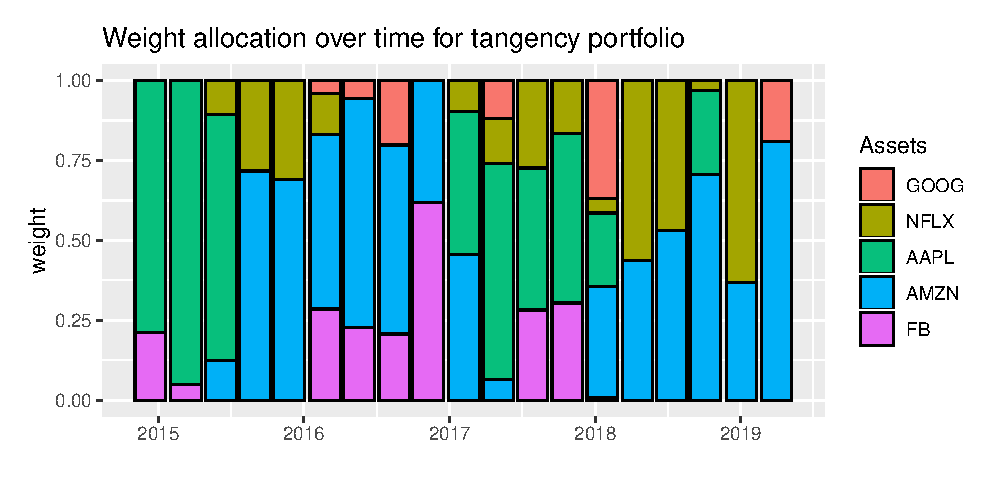
\includegraphics[scale=.7]{codes/weights-msr.eps}
\end{figure}
\end{frame}


\begin{frame}[fragile]
  \frametitle{Practical Example}
\begin{minted}[
framesep=2mm,
baselinestretch=1.2,
fontsize=\footnotesize,]{R}

backtestChartStackedBar(bt, portfolio = "risk parity",
                        legend = TRUE)
\end{minted}
\begin{figure}[!htb]
  \centering
  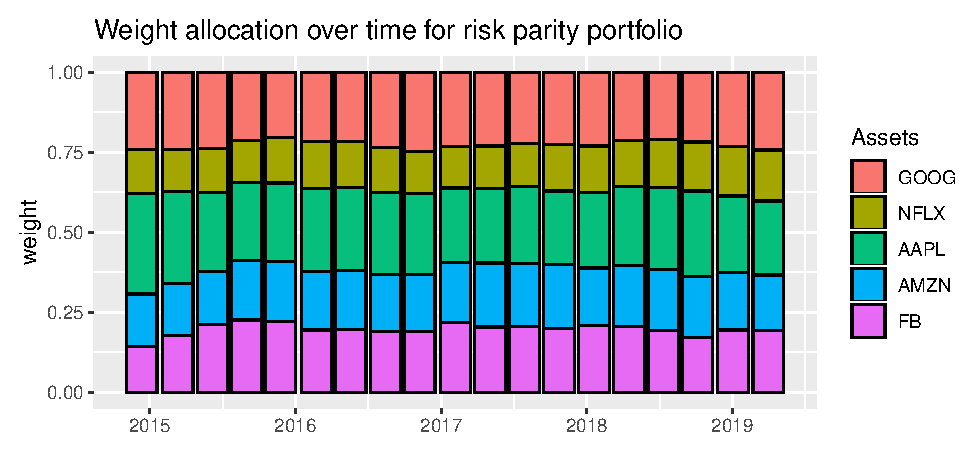
\includegraphics[scale=.7]{codes/weights-rpp.eps}
\end{figure}
\end{frame}


\begin{frame}[fragile]
\frametitle{Practical Example}
\begin{minted}[
  framesep=2mm,
  baselinestretch=1.2,
  fontsize=\footnotesize,
]{R}
backtestChartCumReturns(bt) + theme(legend.position="top")
\end{minted}
\begin{figure}[!htb]
  \centering
  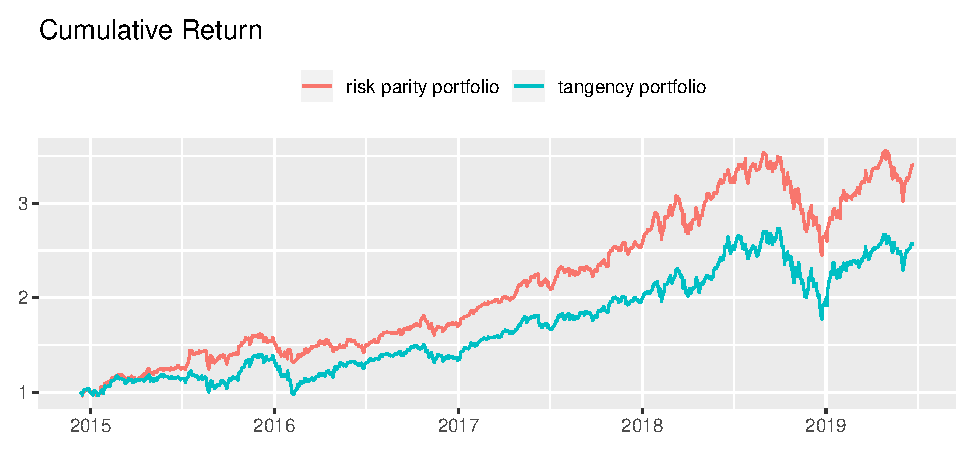
\includegraphics[scale=.7]{codes/returns.eps}
\end{figure}
\end{frame}

\begin{frame}{Testimonials}
  \vspace{.5cm}
  "I can easily run optimizations across new covariance matrices in seconds, which has helped streamline portfolio allocation testing"\linebreak
  \begin{flushright}Jonathan Dane, CFA. Director of Portfolio Strategy \& Market Research, The Coury Firm.\end{flushright}

    "\textbf{riskParityPortfolio} provides a state-of-the-art
   implementation of rpps, otherwise only available at the top quantitative
   hedge funds"\linebreak
   \begin{flushright}Tharsis Souza, PhD. VP at TwoSigma. Founder, OpenQuants.com.\end{flushright}

   {\footnotesize Disclaimer: views, thoughts, and opinions expressed in the text belong solely to the author,
   and not necessarily to the author’s employer, organization, committee or other group or individual.}
\end{frame}

\section{Hierachical Risk Parity}

\begin{frame}{Graph Theory 101}
  \vspace{.5cm}

  \begin{tabular}{cl}
          \begin{tabular}{l}
             \parbox{0.5\linewidth}{
               %  change the parbox width as appropiate
  \begin{itemize}
    \item A graph $\mathcal{G} = \left(\mathcal{V}, \mathcal{E}, \bm{W}\right)$
      \pause
    \item Vertex set $\mathcal{V} = \left\{1, 2, \dots, p\right\}$
      \pause
    \item Edge set $\mathcal{E} \displaystyle \subseteq \left\{\left\{u, v\right\}: u,v \in \mathcal{V}\right\}$
      \pause
    \item Weighted adjacency matrix $\bm{W}$, $\bm{W} \in \mathbb{R}_{+}^{p\times p}$
      \pause
     \begin{itemize}
       \item $W_{ii} = 0, W_{ij} > 0 ~\text{iff}~ \{i,j\} \in \mathcal{E}, W_{ij} = 0~\text{otherwise}$
      \pause
       \end{itemize}
  \end{itemize}
    }
  \end{tabular} &
         \begin{tabular}{l}
    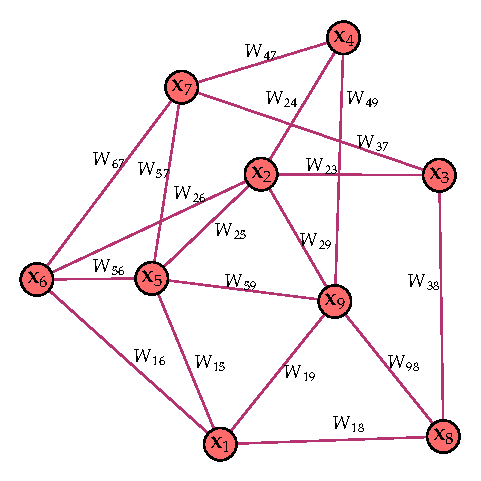
\includegraphics[scale=0.65]{images/graph-with-edge-label.eps}
          \end{tabular}
  \\
\end{tabular}
\end{frame}

\begin{frame}{Graph Theory 101: Tree graph}
  \vspace{.5cm}
  \begin{itemize}
    \item Tree graph: fully-connected graph such that $|\mathcal{E}| = p-1$
    \pause
  \end{itemize}
  \begin{figure}
    \centering
    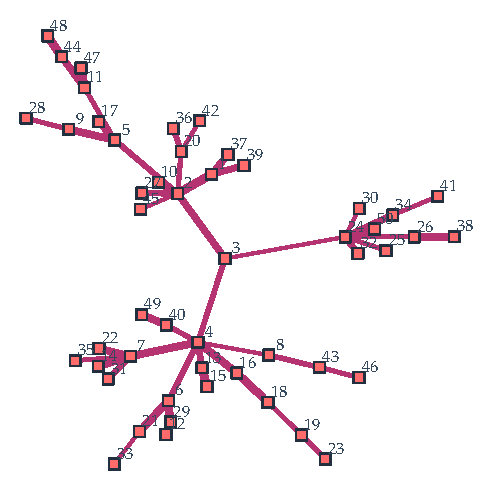
\includegraphics[scale=0.45]{images/tree-original.eps}
    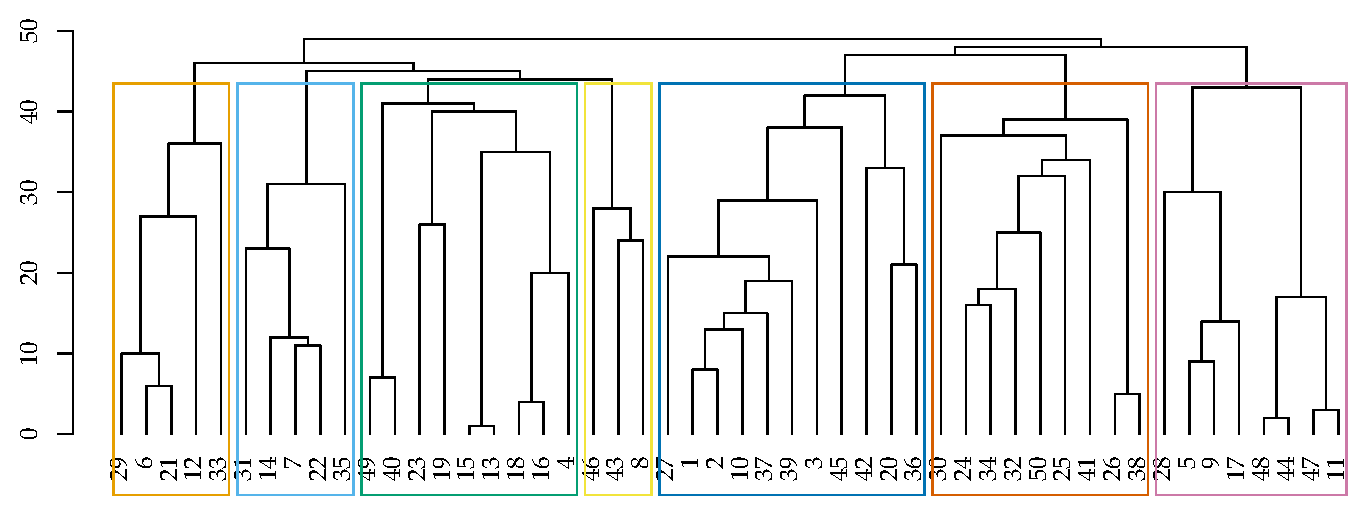
\includegraphics[scale=0.45]{images/dendogram-original.eps}
  \end{figure}
\end{frame}

\begin{frame}{Graph Theory 101: Minimum Spanning Tree}
  \vspace{.5cm}
\begin{tabular}{cl}
        \begin{tabular}{l}
           \parbox{0.5\linewidth}{
  \begin{itemize}
    \item \textbf{def}: an MST of a graph $\mathcal{G}$ is a tree graph spans $\mathcal{G}$ with the minimum possible sum of edge weights
    \item An MST is \textbf{unique} as long as the edge weights are distinct
  \end{itemize}
     }
  \end{tabular} &
         \begin{tabular}{l}
    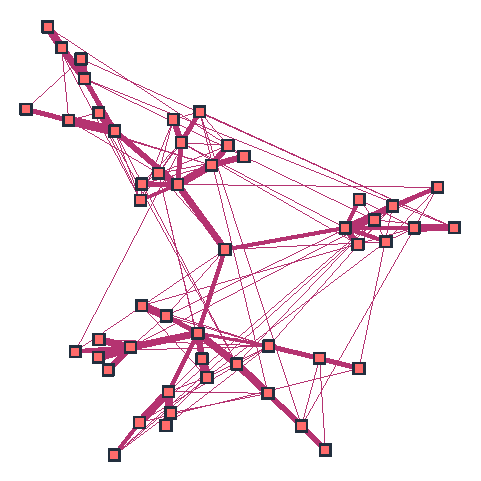
\includegraphics[scale=0.65]{images/mst-example.eps}
          \end{tabular}
  \\
\end{tabular}
\end{frame}

\begin{frame}{Graph Theory 101: Minimum Spanning Tree}
  \vspace{.5cm}
\begin{algorithm}[H]
  \caption{BuildMST (Kruskal's algorithm)}
    \SetAlgoLined
    \KwData{Distances between nodes $\left\{{d}_{ij}\right\}_{1 \leq i, j \leq p}$}
    \KwResult{$\mathcal{G}_{\mathsf{MST}}$}
    $\triangleright$ \text{start with an empty graph} $\mathcal{G}_{\mathsf{MST}} \leftarrow (\mathcal{V}_{\mathsf{MST}}, \mathcal{E}_{\mathsf{MST}})$ \\
    $\mathcal{E}_{\mathsf{MST}} \leftarrow \emptyset$\\
    $\mathcal{V}_{\mathsf{MST}} \leftarrow \{i\}_{1 \leq i \leq p}$\\
    \For{$\{i, j\} \in \mathcal{V}^2_{\mathsf{MST}}$ ordered by increasing $d_{ij}$}{
      $\triangleright$ \text{Verify that $i$ and $j$ are not already connected by a path} \\
      \If{\textbf{not} $\mathsf{connected}(i, j)$}{
      $\mathcal{E}_{\mathsf{MST}} \leftarrow \mathcal{E}_{\mathsf{MST}}\cup\left\{\left\{i, j\right\}\right\}$
      }
    }
\end{algorithm}
\end{frame}

\begin{frame}{Hierarchical Risk Parity}
  \vspace{.5cm}
  \begin{itemize}
    \item \textbf{problem:} modern portfolio theory is sensitive to estimation errors on $\boldsymbol\mu$ and $\boldsymbol\Sigma$
  \end{itemize}
  \pause
  \begin{itemize}
  \pause
    \item Alternatives:
      \begin{itemize}
        \item Robustness
  \pause
        \item Bayesian priors, e.g., Black and Litterman
  \pause
        \item Improving inverse covariance matrix estimation, e.g., Ledoit and Wolf
      \end{itemize}
  \end{itemize}
  \pause
  \begin{itemize}
    \item HRP idea: exploit the intrinsic hierarchy of the correlation matrix
  \pause
    \item weights are allocated in a top-down fashion, just like how asset managers build their portfolios, e.g., from asset class, to sectors, to individual securities
  \end{itemize}
\end{frame}

\begin{frame}{Hierarchical Risk Parity}
  \vspace{.5cm}
  The HRP algorithm proposed by Lopez de Prado, 2016, has basically two steps:
  \begin{enumerate}
  \pause
    \item Build an MST with input matrix: $d_{ij} = \sqrt{\frac{1}{2}(1 - \rho_{ij})}$, where $\rho_{ij}$ is the correlation between stock $i$ and $j$
  \pause
    \item Use \textbf{Recursive Bisection} to allocate the portfolio weights
  \end{enumerate}
\end{frame}
\begin{frame}{Hierachical Risk Parity}
  \vspace{.5cm}
  \begin{algorithm}[H]
    \scriptsize
  \caption{Recursive Bisection}
    \SetAlgoLined
    \KwData{Distances between nodes $\left\{{d}_{ij}\right\}_{1 \leq i, j \leq p}$, estimated covariance matrix $\boldsymbol\Sigma$}
    \KwResult{Portfolio allocation $\bm{w}$}
    $\triangleright$ Initialization \\
    \hspace{.5cm} $\bullet$ set the list of items $L = \{L_{0}\}$, with $L_{0} = \{i\}_{i=1, \dots, p}$ according to the order obtained by the dendogram\\
    \hspace{.5cm} $\bullet$ assign a unit weight to all assets: $w_i = 1, ~\forall~ i = 1, \dots, p$\\
    $\triangleright$ if $\vert L_i \vert = 1,~\forall ~L_i \in L$ then stop.\\
    $\triangleright$ for each $L_i \in L$ such that $\vert L_i\vert$:\\
    \hspace{.5cm} $\bullet$ bisect $L_i$ into two subsets, $L_i^{(1)} \cup L_i^{(2)} = L_i$, where $\vert L_i^{(1)}\vert = \mathsf{round}(\frac{1}{2}\vert L_i\vert)$, and the order is preserved \\
    \hspace{.5cm} $\bullet$ define the variance of $L_{i}^{(j)}$ as $\tilde{\sigma}_{i}^{(j)} = (\theta^{(j)}_{i})^\top \boldsymbol\Sigma^{(j)}_{i} \theta^{(j)}_{i}$,
    where $V^{(j)}_{i}$ is the covariance matrix between the constituents of the $L^{(j)}_{i}$ bisection and $\theta^{(j)}_{i}$ are the inverse variance weights\\
    \hspace{.5cm} $\bullet$ compute the split factor $\alpha_i = 1 - \dfrac{\tilde{\sigma}_{i}^{(1)}}{\tilde{\sigma}_{i}^{(1)} + \tilde{\sigma}_{i}^{(2)}}$\\
    \hspace{.5cm} $\bullet$ re-scale allocations $\bm{w}_{l}$ by a factor of $\alpha_i, ~\forall~ l \in L^{(1)}_i$\\
    \hspace{.5cm} $\bullet$ re-scale allocations $\bm{w}_{l}$ by a factor of $1 - \alpha_i, ~\forall~ l \in L^{(2)}_i$\\
    go to \textbf{4}
  \end{algorithm}
\end{frame}

\begin{frame}{Hierachical Risk Parity}
  \begin{center}
  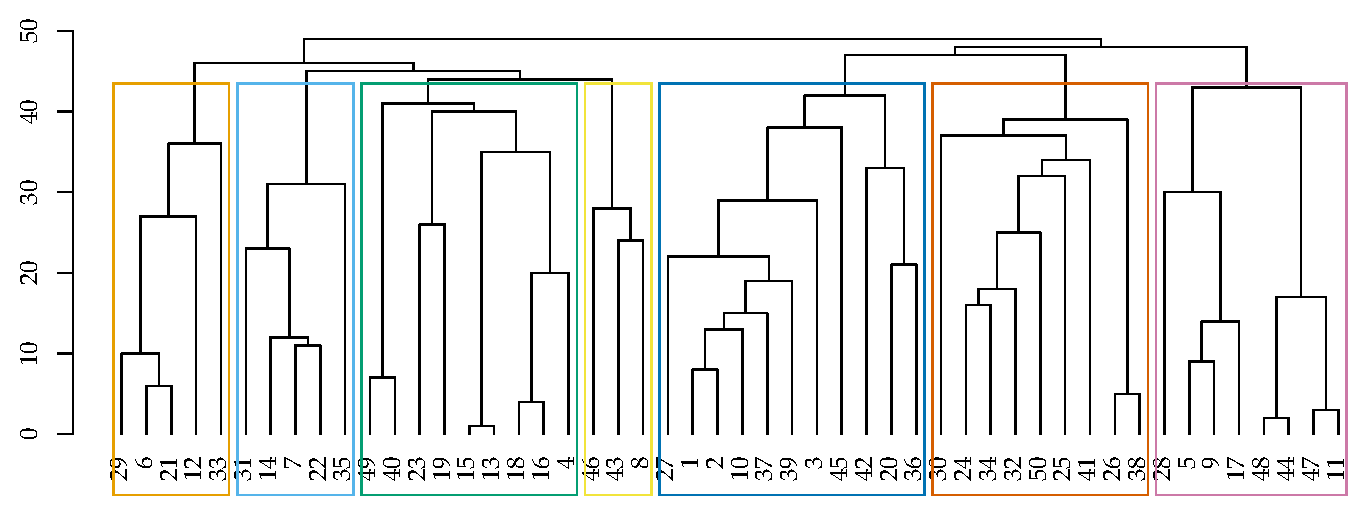
\includegraphics[scale=.65]{images/dendogram-original.eps}
  \end{center}
\end{frame}

\begin{frame}[fragile]
  \frametitle{HRP in Practice}
  \begin{itemize}
    \item $\mathsf{pip~install~\textbf{mfinlab}}$
\end{itemize}

\begin{minted}[
  frame=lines,
  framesep=2mm,
  baselinestretch=1.2,
  fontsize=\footnotesize,
  ]{python}
from mlfinlab.portfolio_optimization.hrp import HierarchicalRiskParity

prices = pdr.get_data_yahoo(stocks_, start="2018-12-31",
                            end="2019-12-31")[['Adj Close']]
hrp = HierarchicalRiskParity()
hrp.allocate(asset_prices=prices)
hrp_weights = hrp.weights
\end{minted}
\end{frame}

\begin{frame}
  \frametitle{HRP in Practice}
  \begin{figure}
  \pause
    \includegraphics[scale=.5]{images/rpp_allocation.eps}
  \pause
    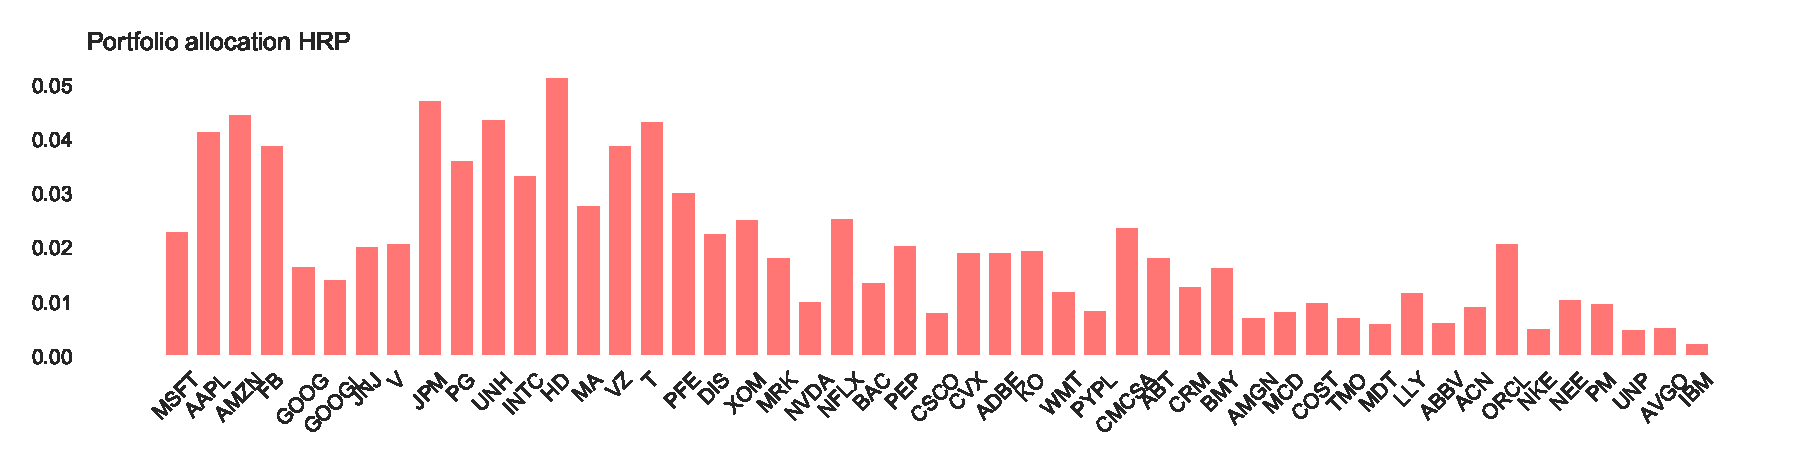
\includegraphics[scale=.5]{images/hrp_allocation.eps}
  \end{figure}
\end{frame}


\begin{frame}
  \frametitle{HRP in Practice}
  \begin{figure}
    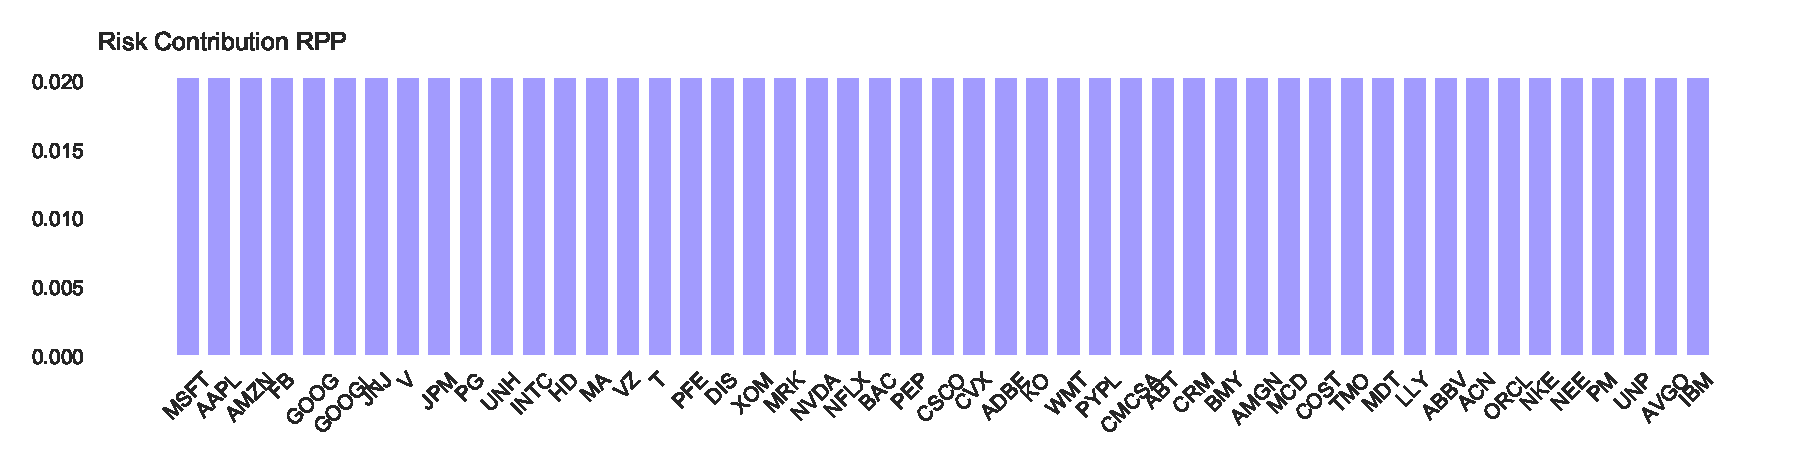
\includegraphics[scale=.5]{images/risk_contrib_rpp.eps}
  \pause
    \includegraphics[scale=.5]{images/risk_contrib_hrp.eps}
  \end{figure}
\end{frame}


\begin{frame}
\frametitle{HRP in Practice}
Now, let's evaluate those portfolios during the COVID-19 2020 crisis:
\pause
\begin{figure}
  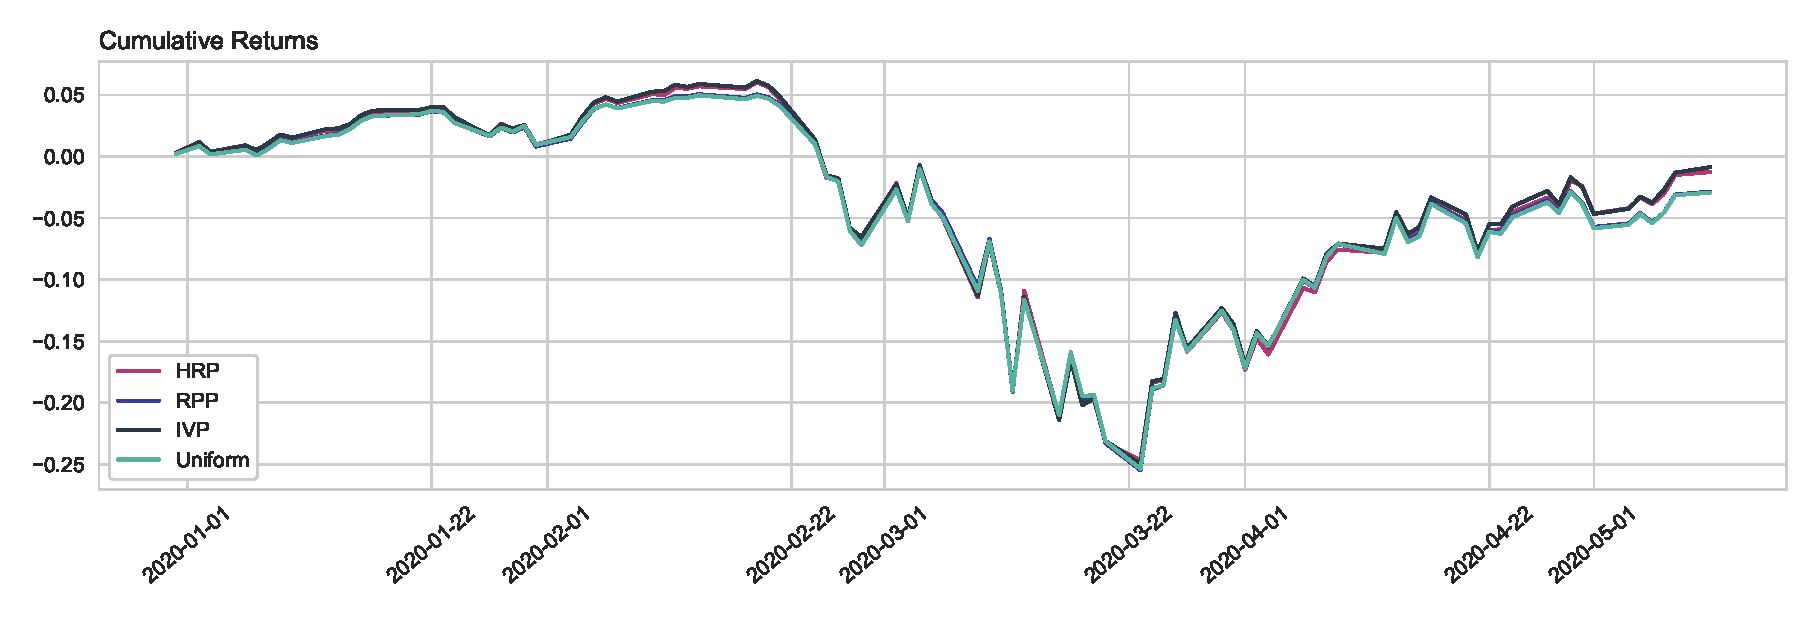
\includegraphics[scale=.5]{images/cum_returns.eps}
\end{figure}
\end{frame}

\begin{frame}{Takeaways}
  \vspace{.5cm}
  \begin{enumerate}
    \item risk parity represents a shift from \textbf{capital} allocation to \textbf{risk} allocation
            \pause
        \vspace{.25cm}
    \item non-convex? no problem!
            \pause
        \vspace{.25cm}
    \item hierarchical risk parity provides a natural way to apply graph theory in portfolio allocation
    \item GitHub repositories to stay tuned:
      \begin{itemize}
        \item dppalomar/riskParityPortfolio
        \item dppalomar/riskparity.py
        \item dppalomar/portfolioBacktest
      \end{itemize}
  \end{enumerate}
\end{frame}

\section{Thank you! Questions?}

\begin{frame}{References}
  \vspace{.5cm}
  \begin{itemize}
    \item {\footnotesize H .M. Markowitz. "Portfolio selection". The Journal of Finance. 7 (1): 77–91, 1952.}
    \item {\footnotesize Y. Feng and D. Palomar, "SCRIP: Successive convex optimization methods for risk parity portfolios design,"
           IEEE Trans. Signal Process., vol. 63, no. 19, pp. 5285–5300, 2015.}
    \item {\footnotesize Scutari et al. "Decomposition by partial linearization: Parallel optimization of multi-agent systems".
           IEEE Trans. Signal Processing, 62(3), 641–656, 2014.}
    \item {\footnotesize B. Bruder and T. Roncalli, "Managing risk exposures using the risk budgeting approach".
           University Library of M\"unich, Germany, Tech. Rep., 2012.}
    \item {\footnotesize F. Spinu, "An algorithm for computing risk parity weights". SSRN, 2013.}
    \item {\footnotesize T. Griveau-Billion, "A fast algorithm for computing high-dimensional risk parity portfolios".
           \url{https://www.thierry-roncalli.com/download/CCD-Risk-Parity.pdf}, 2013.}
    \item {\footnotesize T. Souza, "DIY Ray Dalio ETF: How to build your own Hedge Fund strategy with risk parity portfolios".
           \url{https://www.openquants.com}}
  \end{itemize}
\end{frame}
\end{document}
